\documentclass[a4paper,12pt,openany]{book}
\usepackage [utf8]{inputenc}
\usepackage [french]{babel}
\usepackage [T1]{fontenc}
\usepackage{listings}
\usepackage{graphicx}
\usepackage{verbatim}

%%configuration de listings
\lstset{
language=c,
basicstyle=\ttfamily\small, 
identifierstyle=\color{red}, 
keywordstyle=\color{blue}, 
stringstyle=\color{black!60}, 
commentstyle=\it\color{green!95!yellow!1}, 
columns=flexible, 
tabsize=1, 
extendedchars=true, 
showspaces=false, 
showstringspaces=false, 
numbers=left, 
numberstyle=\tiny, 
breaklines=true, 
breakautoindent=true, 
captionpos=b
}

%coloration syntaxique
\usepackage{xcolor}
\definecolor{Zgris}{rgb}{0.87,0.85,0.85}

\newsavebox{\BBbox}
\newenvironment{DDbox}[1]{
\begin{lrbox}{\BBbox}\begin{minipage}{\linewidth}}
{\end{minipage}\end{lrbox}\noindent\colorbox{Zgris}{\\usebox{\BBbox}}
[.5cm]}

%Pour l espace entre la section et la chapitre (qui est trop grand).
\usepackage{titlesec}

\titleformat{\chapter}[block]
  {\normalfont\Huge\bfseries}% font of number
  {\chaptertitlename\ \thechapter~:}% format of number
  {20pt}% space between number and title
  {\Huge}% font of title

\titlespacing*{\chapter}
  {0pt}%  indent
  {0pt}% space before
  {20pt}% space after
\titlespacing*{\section}
  {0pt}%  indent
  {3.5ex plus 1ex minus .2ex}% space before
  {2.3ex plus .2ex}% space after

\author{Mendy Fatnassi}
\title{Théorie Des Graphe}




%%%%%%%%%%%%%%%%%%%%%%%%%%%%%%%%%%%%%%	Page	%%%%%%%%%%%%%%%%%%%%%%%%%%%%%%%%%%%%%%%%

\begin{document}
\maketitle
\tableofcontents

\chapter{Les graphes}

Les graphes sont utilisé en mathematique et en informatique.\\
Un graphe G est representer par ces \emph{sommet} \textbf{S} et \texbf{A} des relations entre ces sommet qu'on appele \emph{arcs} , on le note donc $G=<S,A>$ .\\
\\
\underline{Vocabulaire}:\\
\\
\textbf{Densité} d'un graphe: Représente un nombre compris entre [0,1.] et se note:\\
\textbf{Orienté}: $D=\frac{A}{S(S-1)}$ \emph{ou} \textbf{Non-Orienté}: $D=\frac{A}{\frac{S(S-1)}{2}}$ (!Ne marche pas avec un graphe a 1 sommet).\\
\\
\textbf{Graphe Simple}: Graphe dans lequel chaque paire de sommets est reliée par au plus une arête et aucun sommet ne possède de boucle.\\
\\
\textbf{Multigraphe}: A l'inverse du graphe simple (simple graph), le multigraphe (multigraph) est un graphe qui autorise des liens multiples (aussi appelés liens parallèles). En d'autres termes, dans un multigraphe, deux sommets peuvent être connectés par plus d'un lien.\\
\\
\newpage
Exemple graphe Simple/Multigraphe:\\
\\
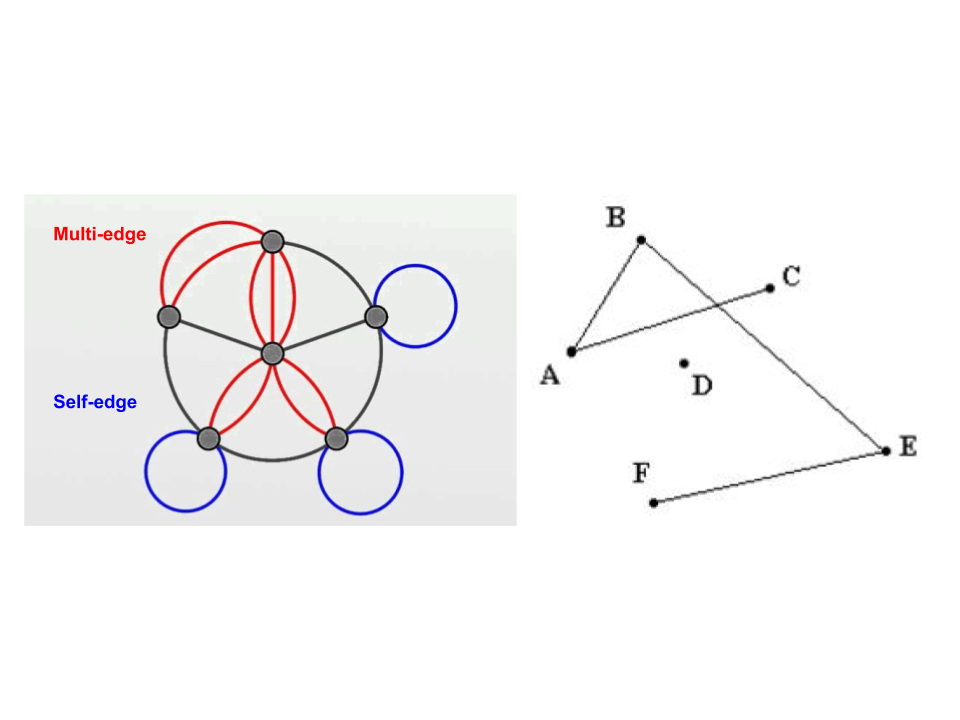
\includegraphics[width=0.5\linewidth,center]{img/simple-multigraphe.png}
\\
\textbf{Graphe Complet}: C'est un graphe simple qui a toutes ses arretes (ou arc) relier. Les graphes K3,3;K4 et K5 sont es graphes complet (\emph{cf.Graphe Planaire}).\\

%%%%%%%%%%%%%%%%%%%%%%%%%%%%%%%%%%%%%%%%%%%%%%%%%%%%%%%%%%%%%%%%%

\section{Graphe Orienté/Non-Orienté}
Un graphe peux etre soit:\\
\\
-\textbf{Non-Orienté} cad que les sommets seront liée simplement par un trait il n'y a pas de sens pour aller d'un sommet quelconque vers un autres.\\
\\
-Une \textbf{aretes}: ensemble fini de paires de sommets.\\ 

-Une \textbf{chaine}: relie un sommet S0 a un sommet Sn correspondant a une suite de sommets ou deux element successif sont relier par une arete.\\

-Un \textbf{cycle}: est une chaine de longueur non nulle reliant un sommet a lui meme.\\
\\
\\
-\textbf{Orienté} c'est a dire qu'il y a un sens de parcours du graphe , les trait seront representer par des flèches .\\
\\
-Un \textbf{arcs}: ensemble fini de couples de sommets.\\ 

-Un \textbf{chemins}: relie un sommet S0 a un sommet Sn correspondant a une suite de sommets ou deux element successif sont relier par un arc .\\

- Un \textbf{circuit}: est un chemin de longueur non nulle reliant un sommet a lui meme .\\
\\
\underline{Exemple}: \\
\\
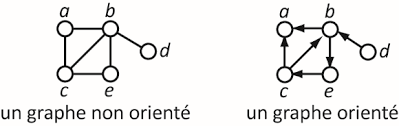
\includegraphics[width=0.5\linewidth,center]{img/gr_n_oriente.png}\\
\\
Longueur d'un chemin (chaine): Nombre d'arcs(aretes) empruntés .\\
Chemin elementaire: Chemin dont tous les sommets sont distincts.\\

%%%%%%%%%%%%%%%%%%%%%%%%%%%%%%%%%%%%%%%%%%%%%%%%%%%%%%%%%%%%%%%%%%%%%%%%%%%%%%%%%%%%%%%%%%%%%%%%%%%%%%%

\section{Connexité/Forte Connexité}

\underline{Vocabulaire}:\\
\\
- Un sous-graphe correspond au graphe de départ moins certain sommet.\\
On le notera S'(prime).\\
- Un graphe partiel correspond au graphe initiale moins certain liens.\\
- Un sous-graphe partiel : S' < S moins certain liens.\\

\textbf{Connexe}: \\
Un graphe non-orienté est connexe si toute paires de sommets distincts est reliée par une chaine.\\
\\
\textbf{Fortement Connexe}:\\
Un graphe orienté est fortement connexe si tout couple de sommets distincts est reliée par un chemin.\\
Il existe un chemin de tout sommet i vers j et inversement.\\

%%%%%%%%%%%%%%%%%%%%%%%%%%%%%%%%%%%%%%

\subsection{Composante Connexe/Fortement Connexe}

\textbf{Composante Connexe (CC)} :\\
Un sous-graphe d'un graphe non-orienté est une composante connexe , si il est connexe et si il est maximal. Un sous-graphe connexe est maximal si on ajoute un sommet dans ce sous-graphe et qu'il n'est plus connexe .\\
Une composante connexe est donc un sous-graphe connexe maximal.\\
\\
\textbf{Composante Fortement Connexe CFC)} :\\
Un sous-graphe d'un graphe orienté est une composante fortement connexe , si il est fortement connexe et si il est maximal. Un sous-graphe connexe est maximal si on ajoute un sommet dans ce sous-graphe et qu'il n'est plus connexe .\\
On peux trouver une chemin de i vers j et inversement .\\
\\
\underline{Tableau recapitulatif des terminologie}:\\
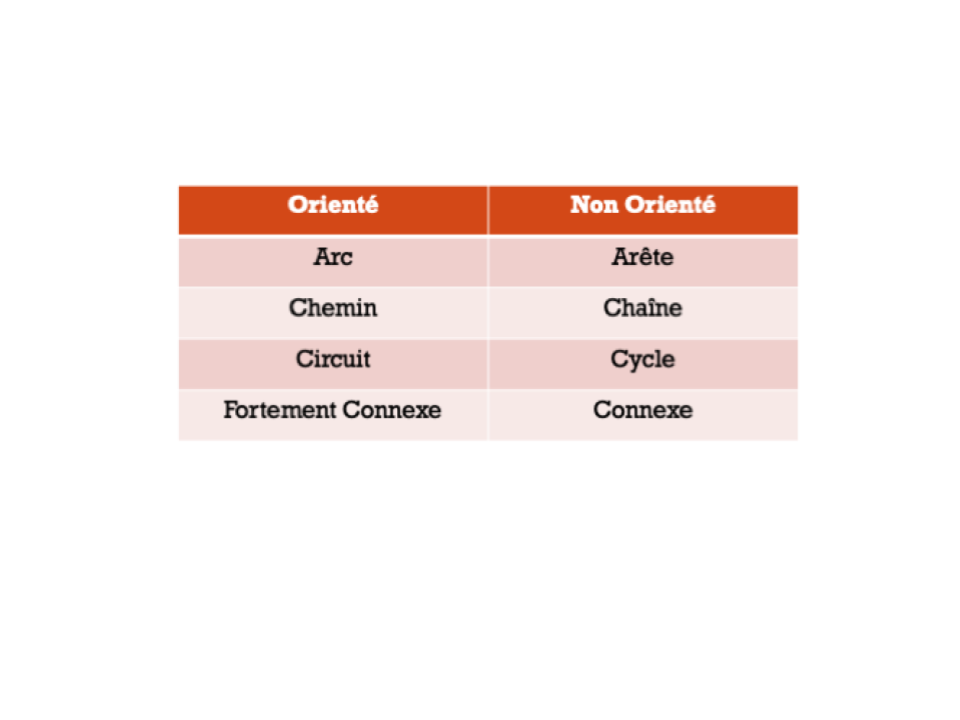
\includegraphics[width=0.75\linewidth,center]{img/tab-graphe-(non)oriente.png}

%%%%%%%%%%%%%%%%%%%%%%%%%%%%%%%%%%%%%%%%%%%%%%%%%%%%%%% Coloriage %%%%%%%%%%%%%%%%%%%%%%%%%%%%%%%%%%%%%%%%%%%%%%%%%%%%%%%

\chapter{Parcours de graphe}

\section{Parcours Eulerien}

Un parcours eulerien passe par chaque arrete du graphe (pas forcément une 1 seul fois).\\
\\
\underline{\textbf{Théoreme d'euler}}: \\
Si le nombre de sommet de degré impair est egale a :\\
- 0: Il existe un cycle solutions\\
- 2: Il existe toujoure une chaine qui vas d'un sommet impair vers un autre sommet impair\\
Sinon il n'y a pas de solution.\\

%%%%%%%%%%%%%%%%%%%%%%%%%%%%%%%%%%%%%%%%%%%%%%%%%%%%%%%

\section{Parcours Hamiltonien}

Un parcours hamiltonien passe par chaque arréte 1 seul fois.\\



%%%%%%%%%%%%%%%%%%%%%%%%%%%%%%%%%%%%%%%%%%%%%%%%%%%% Graphe Planaire %%%%%%%%%%%%%%%%%%%%%%%%%%%%%%%%%%%%%%%%%%%%%%%%%%%%%%

\chapter{Graphe Planaire}

Un graphe est dit planaire si on peux le dessiner sur un plans et n'ayant aucun croisement.\\
\\
\underline{\texbf{Théoreme de Kuratowski}}: \\
Un graphe est planaire si et seulement si il ne contient aucun sous-graphe reductible a K3,3 ou K5.\\
\\
Voici un exemple de graphe K3,3 , K4 et K5 qui d'ailleur sont des graphes complet:\\
\\
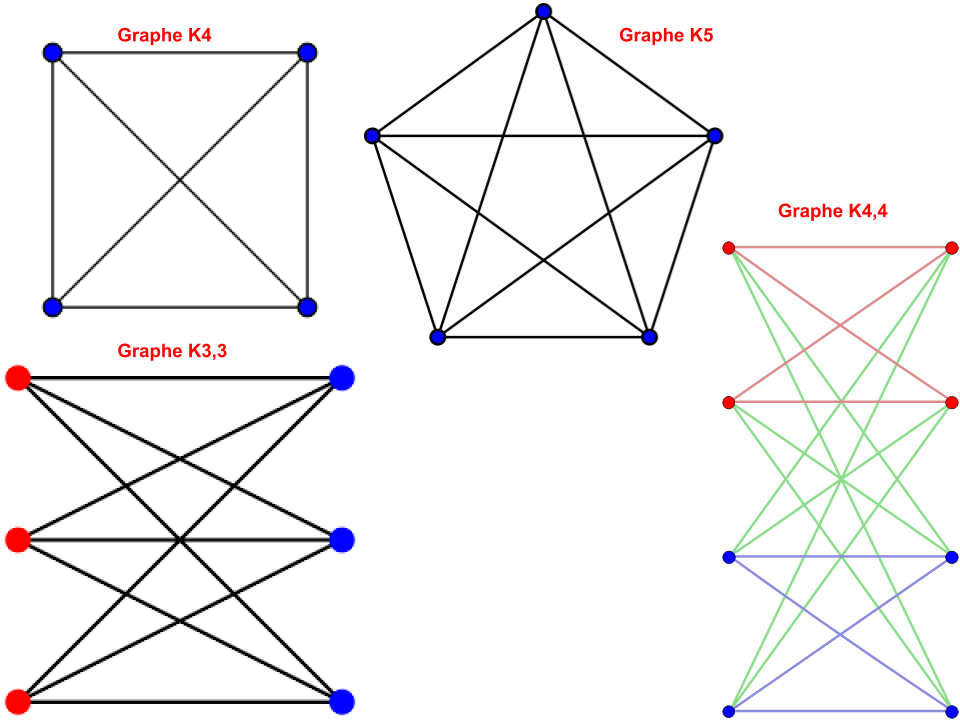
\includegraphics[width=0.6\linewidth,center]{img/graph-K.png}



%%%%%%%%%%%%%%%%%%%%%%%%%%%%%%%%%%%%%%%%%%%%%%%%%%%%%%%% Bipartie %%%%%%%%%%%%%%%%%%%%%%%%%%%%%%%%%%%%%%%%%%%%%%%%%%%%%%

\chapter{Bipartisme}

\section{Affectation de registre}

L'affectation de registre dans un graphe revient a traité un probléme de coloriage de graphe.\\
Pour savoir quelle info doit etre traité avant (Si c'est plus important ou non).\\
\\
Pour savoir combien de registre on vas affecter au graphe nous allons essayé de le colorier avec le moins de couleur(registre) possible.\\
On a une régle a respecter: On ne peux pas avoir cote-a-cote une meme couleur.\\
\\
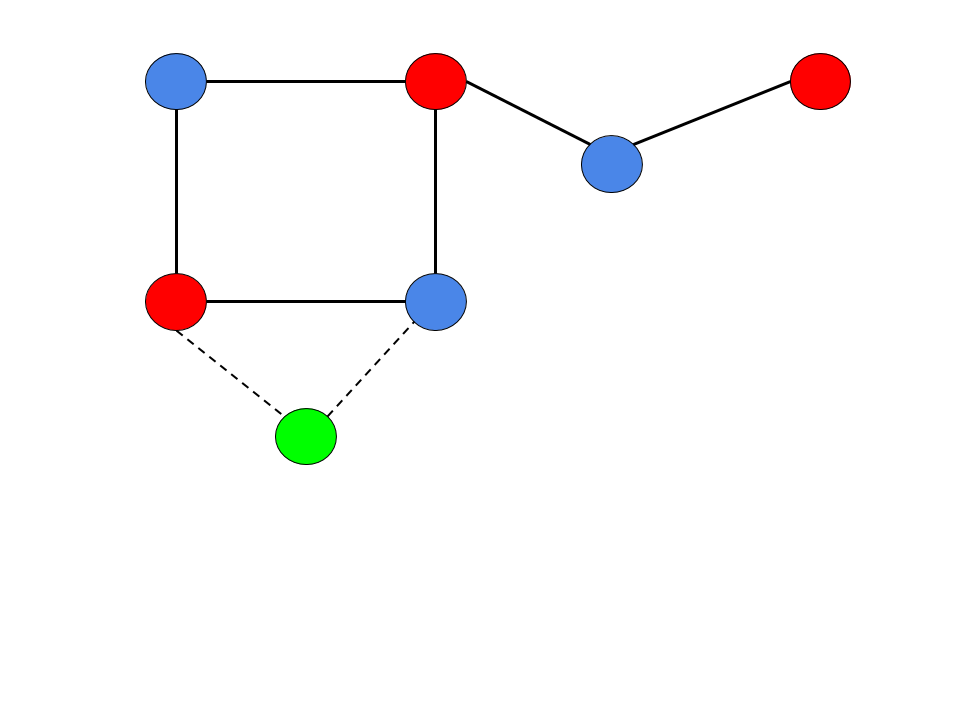
\includegraphics[width=0.5\linewidth,center]{img/graphe-bicolore.png}

%%%%%%%%%%%%%%%%%%%%%%%%%%%%%%%%%%%%%%%%%%%%%%%%%%%%%%%%

\subsection{Algorithme Heuristique}

\begin{verbatim}
rep
  x <- sommet+haut degré
  empiler                                 // Detruie G
  G <- G\{x}
frep

rep
  x <- depiler()
  colorier                                // Construire G
  G <- G U {x}
frep
\end{verbatim}

%%%%%%%%%%%%%%%%%%%%%%%%%%%%%%%%%%%%%%%%%%%%%%%%%%%%%%%%

\subsection{Graphe Bipartie}

Un graphe est dit biparti si on peut partager son ensemble de sommets en deux parties A et B tels qu'il n'y ait aucune arête entre éléments de A et aucune arête entre éléments de B.\\
\\
Autrement dit, les graphes bipartis sont ceux que l'on peut colorer en utilisant au plus deux couleurs. Le théorème suivant, dû à König en 1916, caractérise les graphes bipartis :\\
\\
\textbf{Théorème de konig}: Un graphe est biparti si et seulement s'il ne contient pas de cycles de longueur impaire.\\
\\
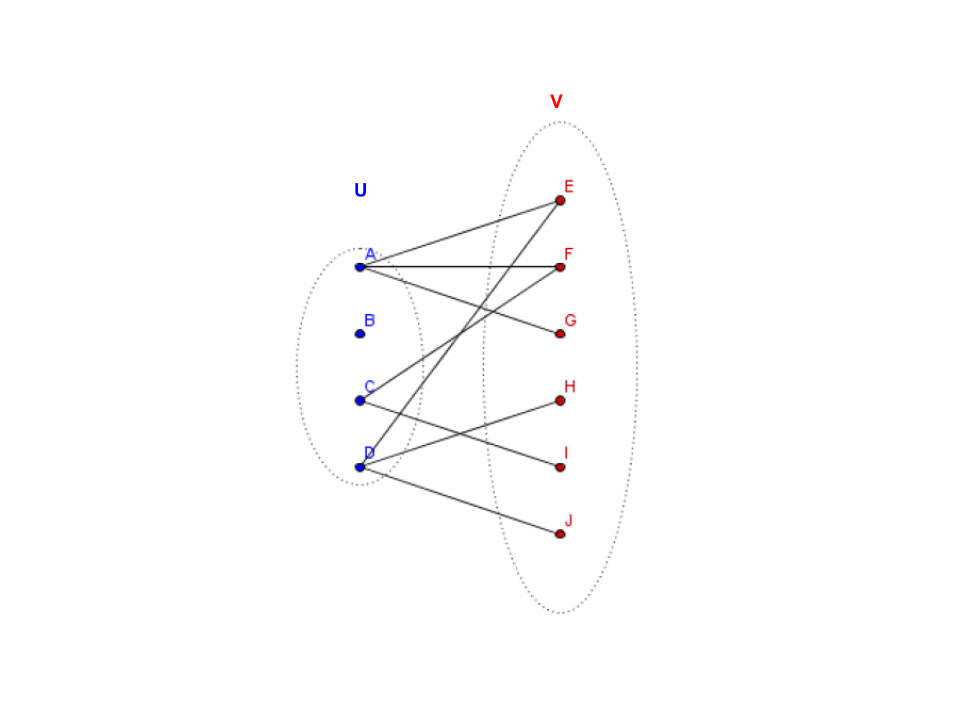
\includegraphics[width=1\linewidth,center]{img/g-bipartie.png}
\\
Rappelons que la longueur d'un cycle est égale au nombre d'arêtes qu'il contient. En particulier, d'après le théorème précédent, les arbres sont des graphes bipartis.



%%%%%%%%%%%%%%%%%%%%%%%%%%%%%%%%%%%%%%%%%%%%%%%%%%% Structure et Algos %%%%%%%%%%%%%%%%%%%%%%%%%%%%%%%%%%%%%%%%%%%%%%%%%%%%

\chapter{Structure et algos de base}

\underline{Probléme}: On veux enumérer les graphes simple a 8 sommets et 3 couleur par arrete ?\\
\\
Le nombre de graphe seras: 4x4x4....x4=$4^28 = 2^56 = 2^{60-4} = \frac{2^{30}x2^{30}}{2^4} \approx 7.10^{16}$\\
\\
\underline{Hypothése}: Le super ordinateur énumere $2^{30} (10^9)$ graphes par secondes.\\
\\
Temps totale: $\frac{2^{30}}{16} = 67 108 864 sec$ donc en 1 année $=\pi x 10^7$ sec avec une erreur < a 1\% .\\
$t=\frac{\pi x 10^7 x 10^2}{\pi x 16} = \frac{100}{16\pi} année \leqslant 2ans$\\
\\
Il faut donc 2ans pour tout enumérer. L'enumeration n'est donc pas une bonne solution, surtout quand le nombre d'echantillon a traité est grand, on préferera utilisé :\\
-Des Structure de Donnée\\
-Des Algorithme sur les graphes\\
\\
Certain probléme de graphe nécessite beaucoup de temps de calcule, or on veux un resultat cas immédiat (1 semaine au plus) pas dans 2 ou 5ans.\\

%%%%%%%%%%%%%%%%%%%%%%%%%%%%%%%%%%%%%%%%%%%%%%%%%%%%%%%%

\section{Structure}

-Pile ou File -> Dequeu (double queu)\\
-Une dequeu fonctionne soit comme une pile soit comme une file (ne pas melanger cela depend du contexte).\\
\\
Primitive:\\
-empiler(), depiler(), enfiler(), defiler() $=>$ O(1)\\
-cardinal, vide\?, present\? => O(1)\\
\\
-tas monceau (heap) : Maximier, Minimier\\
%inclure exemple de cours feuille

%%%%%%%%%%%%%%%%%%%%%%%%%%%%%%%%%%%%%%%%%%%%%%%%%%%%%%%%

\section{Matrice d'incidence}

\underline{Avantage}: \\
\\
-plus agréable pour l'homme.\\
-ajout/suppression des arcs ne change pas la dimension du tableau.\\
\\
\underline{Inconvénient}:\\
\\
-Traitement en $O(S)^2$\\
-Met plus de temps a trouver l'arc suivant.\\

%inclure exemple de cours feuille plexe


%%%%%%%%%%%%%%%%%%%%%%%%%%%%%%%%%%%%%%%%%%%%%%%%%%%%%%%%%%%%%%%%%%%%%%%%%%%%

\section{Graphe Inverse}

\underline{Principe}: \\
-Determiner la taille de chaque plexe dans H, graphe inverse de G.\\
-Remplir H.Suk et H.Head\\
\\

\subsection{Algos Graphe Inverse}

\begin{verbatim}
//deg[] degrés sortant dans H

Razer (deg)

rep pour k de 1 a G.A   //A:Arrete
  deg[G.Suk[k]]++
frep
//H.Head <-- au dela de chaque bloc

H.Head[0] <- 1

rep x de 1 a G.S      //S:Sommet
  H.Head[x+1] <- H.Head[x]+deg[x]
frep
//H.Suk <-- remplie en marche arriere 

rep x de 1 a G.S
  rep k de G.Head[x] a H.Head[x+1]-1
    y <- G.Suk[k]
    H.Head[x]--
    H.Suk[H.Head[y]] <- x
  frep
frep

//terminer la structure

H.S=G.S
H.A=G.A
H.Head[H.S+1]=H.A+1
H.Head[0]=0
\end{verbatim}
\\
temps totale: O(S+A) , on considére A $\geqslant$ S dans les graphes connexe.\\

%%%%%%%%%%%%%%%%%%%%%%%%%%%%%%%%%%%%%%%%%%%%%%%%%%%%%%%%%%%%%%%%%%%%%%%%%%%%

\section{Tri Topologique}

Les champs sont inversé; Suk devient Kus et Hed devient Deh.\\
Possible si le graphe ne contient pas de circuit.\\

\underline{Principe}:\\
On commence par noté le premier sommet par 1 (ordre croissant), ensuite on marque chaque sommet S si le precedent de S est deja marqué.\\

%%%%%%%%%%%%%%%%%%%%%%%%%%%%%%%%%%%%%%

\subsection{Algos Tri Topologique}
\begin{verbatim}
\\deg[] degré entrant 
Razer(nivo)
Razer(deg)

Rep pour k de 1 a G.A
  deg[Suk[k]]++
Frep

//Initialiser la deque
Rep x de 1 a S
  Si deg[x]==0
    enfiler(x)
  Fsi
  N <- 0
Frep

Rep jusqu'a dequeVide()
  N++

  Rep de 1 a dequeCardinal()
    x <- defiler
    nivo[x] <- N

    Rep pour tout succ de H y de x
      deg[y]--
      Si deg[y]==0
        enfiler(x)
      Fsi
    Frep
  Frep
Frep
\end{verbatim}

%%%%%%%%%%%%%%%%%%%%%%%%%%%%%%%%%%%%%%%%%%%%%%%%%%%%%%%%%%%%%%%%%%%%%%%%%%%%

\section{Exploration de graphe}

Marquae des sommets.\\

%%%%%%%%%%%%%%%%%%%%%%%%%%%%%%%%%%%%%%

\subsection{Algos }
\begin{verbatim}
Next <- Head
Mark <- 0 partout
x <- 1
Mark[x] <- vrai
E <- {x}

Rep jusqu'a E vide
  x <- 1 sommet qlq de E (utile plus tard)

  Si Next[x] < Hed[x+1]
    y <- Next[x]

    Si y non-marqué
      E <- E U {y}
    Fsi
    Next[x]++
    
    Sinon
      E <- E\{x}
  Fsi
Frep
\end{verbatim}

%%%%%%%%%%%%%%%%%%%%%%%%%%%%%%%%%%%%%%%%%%%%%%%% Parcours de graphe %%%%%%%%%%%%%%%%%%%%%%%%%%%%%%%%%%%%%%%%%%%%%%%%%%%
\chapter{Parcours en Profondeur/Largeur}

\section {Parcours en Profondeur}

On prend les sommets par ordre croissant, marqué le 1er sommet  ensuite marqué ces successeur.\\
Si pas de successeur, revenir au sommet precedent (depiler) pour trouver un nouveau successeur tant qu'on est pas arrivée jusqu'a trouvé un nouveau successeur.\\
%inclure exemple feuille cours
\\
Resultat G1: 1,2,3,4 \\
Resultat G2: 1,2,3,4,6 (5,7 et 8 ne font pas partie du parcours) \\
Resultat G3: 1,2,3,4,7,6,10,5,9,8 \\

%%%%%%%%%%%%%%%%%%%%%%%%%%%%%%%%%%%%%%

\section {Parcours en Largeur}

%inclure exemple de cours
Resultat G1: 1|2,3|4|6 \\
Resultat G2: 1|2,3|4|6 \\
Resultat G3: 1|2,5,8|3,6,9|4,7,10 \\



%%%%%%%%%%%%%%%%%%%%%%%%%%%%%%%%%%%%%%%%%%%%%%%%%%%%%%% Distancier %%%%%%%%%%%%%%%%%%%%%%%%%%%%%%%%%%%%%%%%%%%%%%%%%%%%%%%%

\chapter{Distancier}

Un graphe G(S,A), on veut calculerla distance la plus courte entre tous les sommets (X,Y).\\
Changement de représentation des données.\\


\section{Algos Distancier}
\begin{verbatim}
Rep k de 1 a S
  Rep i de 1 a S
    Rep j de 1 a S
      Si D[i,j] > D[i,k]+D[k,j]
        D[i,j] <- D[i,k]+D[k,j]
        P[i,j] <- P[i,k]
      Fsi
    Frep
  Frep
Frep

D[][]

Rep pour i de 1 a S
  D[i][i] <- 0
  Rep j succ h de i dans G
    D[i][j] <- [i][j]
  Frep
Frep
\end{verbatim}
\\

%%%%%%%%%%%%%%%%%%%%%%%%%%%%%%%%%%%%%%%%%%%%%%%%%%%%%%%%%%%%%%%%%%%%%%%%%%%%

\section{Algos Potentiel tache}
Donnée: Un graphe sans circuit , description de tache donnée par G.\\
Resultat: Date au plus tot/tard, Marges, Chemin critique.\\


\chapter{Dijsktra}

\subsection{Plus long chemin}
Il y a une boucle \verb+{2,3,2}+, ducoup pour trouvé le chemin le plus "long" on pourrai basculé a l'infinie or on veux un parcours elemenetaire (1 fois), ducoup pas possiblepour le graphe ci-dessus.\\

\end{document}